Przewodniki tworzenia nowych obiektów zostały oparte o bibliotekę \textbf{Spring WebFlow} (\ref{tech:spring_web_flow}). Każdy z kreatorów opisany jest na trzech płaszczyznach. Jedną z nich jest warstwa widoku. Widok składa się z plików \textbf{JSP}, gdzie każdy z nich zawiera formularz pozwalający na wprowadzenie danych. Relacja między nimi a przewodnikiem opisana jest przez relację jeden do jednego - jeden formularz przypada na jeden plik \textbf{JSP}. Definicja pełnej sekwencji kroków zapisana jest w pliku \textbf{XML}, zrozumiały dla biblioteki \textbf{Apache Tiles}. Po drugiej stronie istnieje natomiast opis przepływu. Przepływ, w rozumieniu biblioteki \textbf{Spring WebFlow}, to sekwencja kolejnych widoków, prezentowanych użytkownikowi oraz możliwych przejść z danego kroku do innych. Trzecia płaszczyzna to klasy języka Java, w których zdefiniowana została logika dla każdego z kroków. Zadaniem tych klas jest przygotowanie danych, które przekazane zostaną do widoku tuż przed jego wyświetleniem, pozwalającym tym samym pokazać elementy takie jak listy rozwijane. Umożliwiają również przetworzenie surowych danych, które użytkownik wprowadził w formularzu, na zrozumiałą dla aplikacji postać. Współpraca wszystkich trzech płaszczyzn zapewniona jest przez bibliotekę \textbf{Spring WebFlow}, która efektywnie mapuje żądania pochodzące od klienta, na, w pierwszej kolejności właściwy moment przepływu, a w dalszej, na klasy obsługujące ten moment. 

\subsection{Kreator nowego szablonu raportu}
\label{wizard:rbuilder}
	\textbf{ReportBuilder} jest narzędziem będącym obecnie w fazie rozwoju, niemniej pozwalającym już teraz na tworzenie raportów biznesowych. Dedykowany dla użytkownika, daje mu możliwość wybrania zbioru interesujących go tabel, kolumn które zebrane razem stanowią logiczny zbiór używany w dalszej kolejności do konstrukcji zapytania do bazy danych i utworzenia gotowego raportu. Przewodnik składa się z 3 kroków:
	\begin{enumerate}
		\item wybranie tabeli lub tabel, dla której wygenerowany zostanie raport
		\item dostosowanie formatowania kolumn,
		\item podanie danych opisujących raport: tytuł, podtytuł, komentarz
	\end{enumerate}			
	
	\begin{figure}[H]
		\centering
		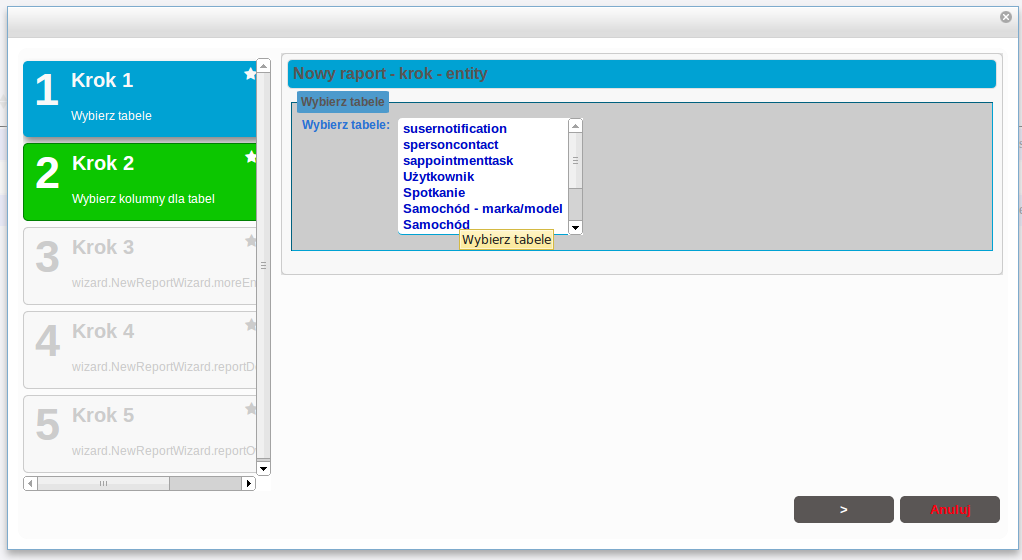
\includegraphics[width=0.80\textwidth]{images/rbuilder_step1}
		\caption[Kreator nowego raportu - krok 1]{Kreator nowego raportu - krok 1, źródło: opracowanie własne}
		\label{app:wizard_newReport_step1}
	\end{figure}	
	\begin{figure}[h]
		\centering
		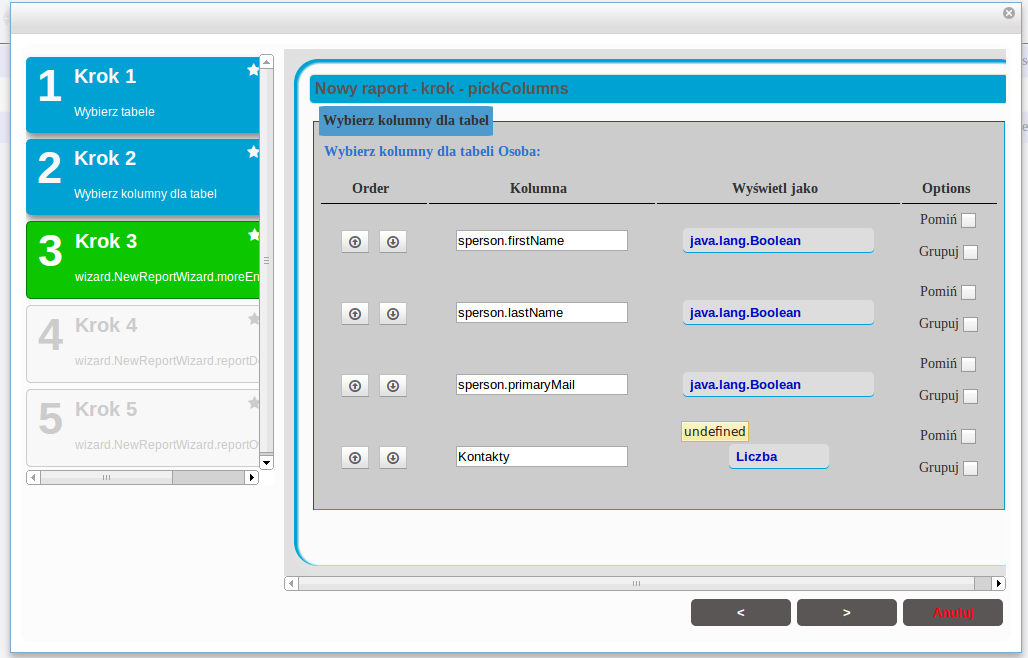
\includegraphics[width=0.80\textwidth]{images/rbuilder_step2}
		\caption[Kreator nowego raportu - krok 2]{Kreator nowego raportu - krok 2, źródło: opracowanie własne}
		\label{app:wizard_newReport_step2}
	\end{figure}		
	\begin{figure}[h]
		\centering
		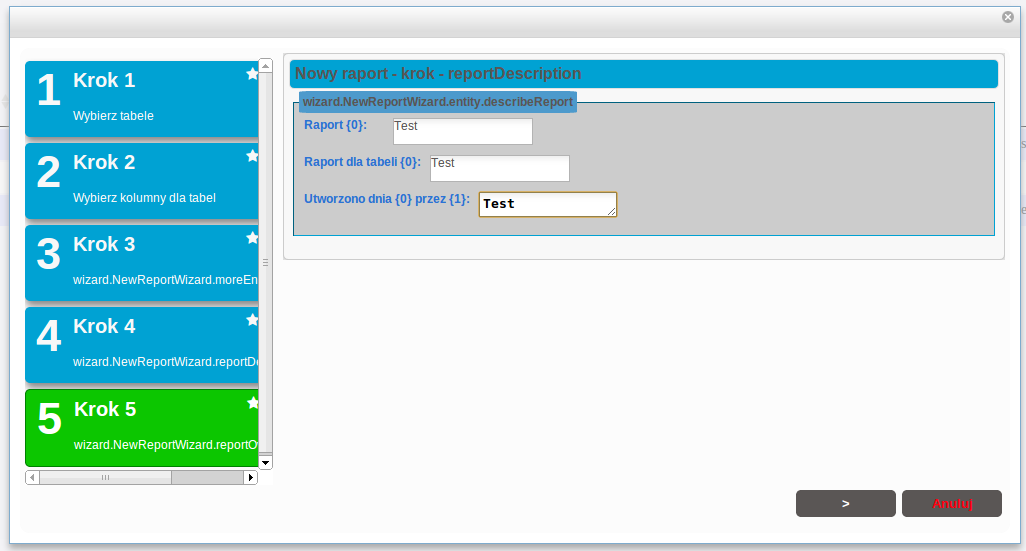
\includegraphics[width=0.80\textwidth]{images/rbuilder_step3}
		\caption[Kreator nowego raportu - krok 3]{Kreator nowego raportu - krok 3, źródło: opracowanie własne}
		\label{app:wizard_newReport_step2}
	\end{figure}		

\subsection{Kreator nowego użytkownika}
	Kreator nowego użytkownika pozwala na tworzenie nowy obiektów klasy \textbf{SUser}. Kwestia uprawnień jest tutaj szczególnie ważna z uwagi na to, że w przewodniku wybiera się zestaw ról. Role, do których przypisany jest użytkownik, stanowią późniejszą bazę do weryfikacji dostępności funkcji systemu dla poszczególnych użytkowników. 
	\begin{figure}[th]
		\centering
		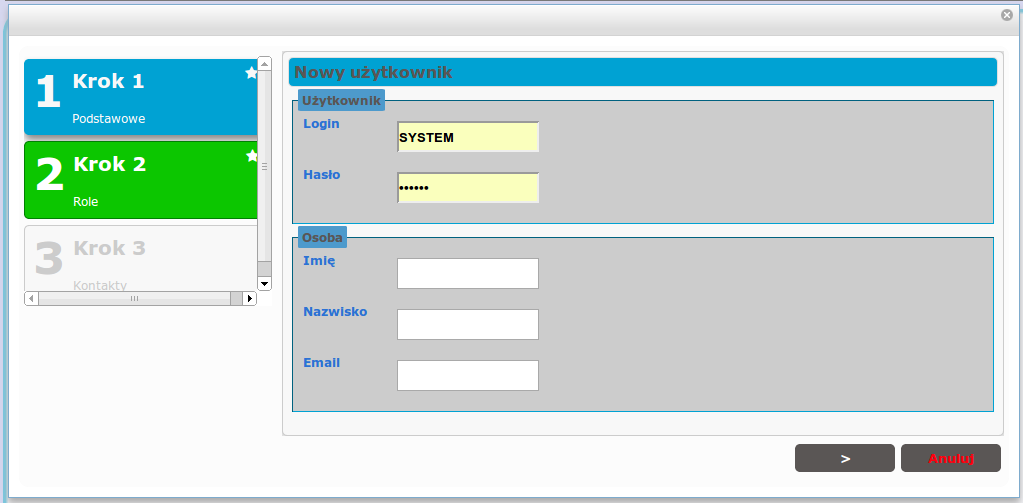
\includegraphics[width=0.8\textwidth]{images/newUser-basic}
		\caption[Kreator nowego użytkownika - dane podstawowe]{
			Kreator nowego użytkownika - dane podstawowe, źródło: opracowanie własne	
		}
		\label{app:newUser_basic}
	\end{figure}	
	\begin{figure}[H]
		\centering
		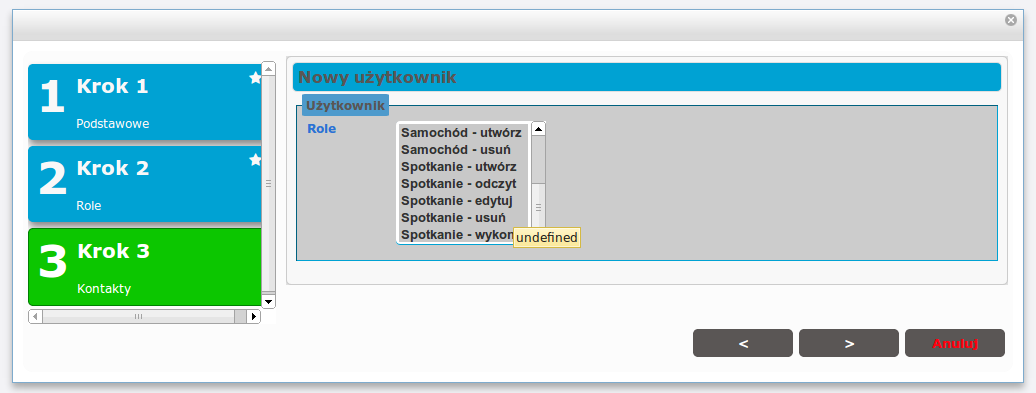
\includegraphics[width=0.8\textwidth]{images/newUser-roles}
		\caption[Kreator nowego użytkownika - uprawnienia użytkownika]{
			Kreator nowego użytkownika - uprawnienia użytkownika, źródło: opracowanie własne
		}
		\label{app:newUser_roles}
	\end{figure}	
	\begin{figure}[th]
		\centering
		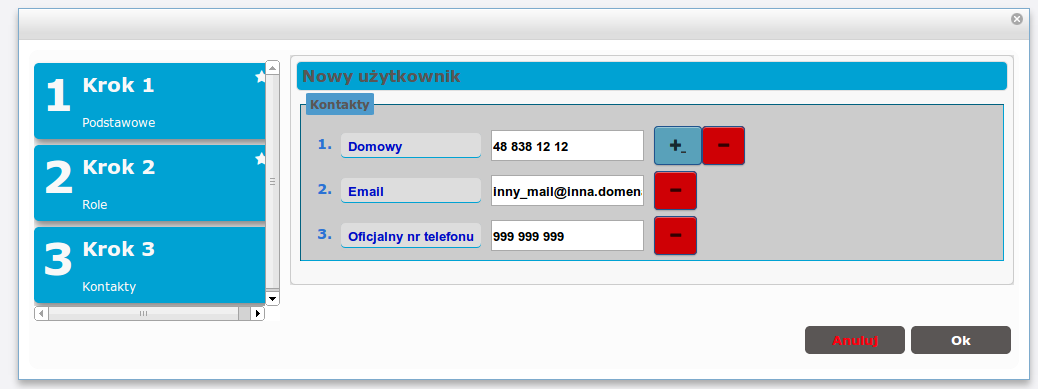
\includegraphics[width=0.8\textwidth]{images/newUser-contacts}
		\caption[Kreator nowego użytkownika - dane kontaktowe]{
			Kreator nowego użytkownika - dane kontaktowe, źródło: opracowanie własne
		}
		\label{app:newUser_contacts}
	\end{figure}	

\subsection{Kreator nowego samochodu}
	Kreator nowego samochodu został zaprojektowany aby tworzyć nowe obiekty klasy \textbf{SCar}.	Pierwszym krokiem jest podanie \textbf{numeru VIN}, z którego system odczytuje wszelkie możliwe dane, które można odkodować korzystając z informacji dostępnych publicznie. Na obecną chwilę są to:
	\begin{itemize}
		\item rok produkcji, zwracany jako lista lat w których samochód mógł być wyprodukowany,
		\item kraj, w którym samochód został wyprodukowany.
	\end{itemize}
	
	W drugim kroku kreator nowego samochodu podaje takie informacje jak:
	\begin{itemize}
		\item markę oraz model,
		\item numer tablicy rejestracyjnej,
		\item rok produkcji,
		\item rodzaj paliwa,
		\item właściciela.
	\end{itemize}
	\begin{figure}[th]
		\centering
		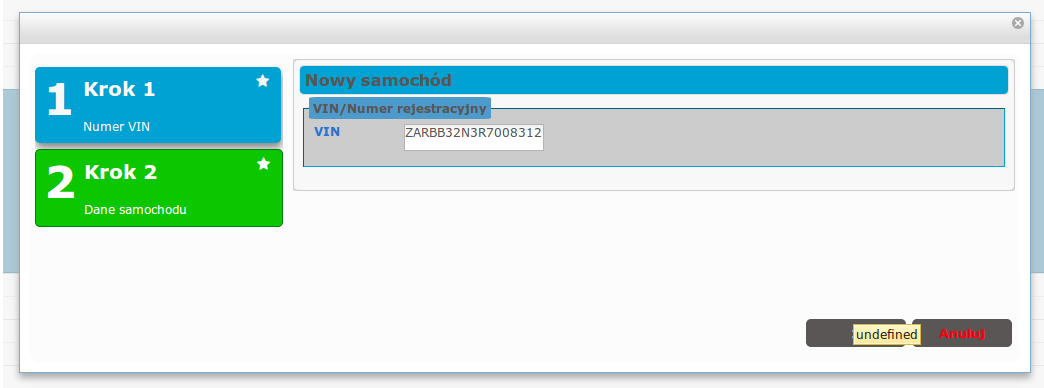
\includegraphics[width=0.9\textwidth]{images/newCar-vin}
		\caption[Kreator nowego samochodu - numer VIN]{
			Kreator nowego samochodu - numer VIN, źródło: opracowanie własne
		}
		\label{app:newCar_vin}
	\end{figure}	
	\begin{figure}[th]
		\centering
		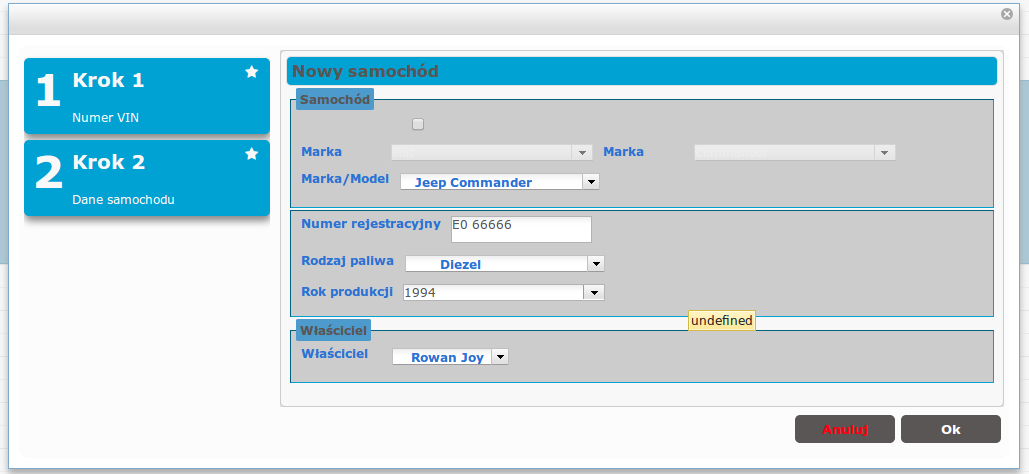
\includegraphics[width=0.9\textwidth]{images/newCar-data}
		\caption[Kreator nowego samochodu - pozostałe dane]{
			Kreator nowego samochodu - pozostałe dane, źródło: opracowanie własne
		}
		\label{app:newCar_data}
	\end{figure}

\subsection{Kreator nowego spotkania}
	
	\begin{figure}[H]
		\centering
		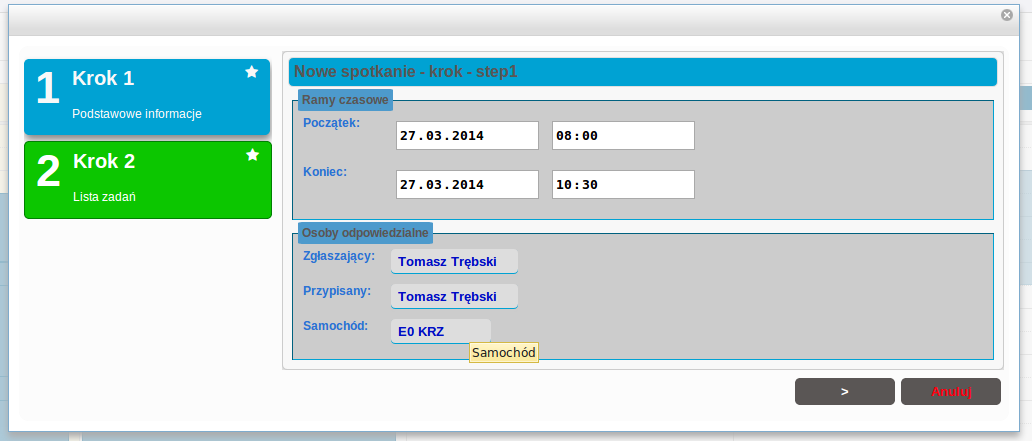
\includegraphics[width=1.0\textwidth]{images/newAppointment_step1}
		\caption[Kreator nowego spotkania - krok 1]{
			Kreator nowego spotkania - krok 1, źródło: opracowanie własne
		}
		\label{app:wizard_newAppointment_step1}
	\end{figure}
	\begin{figure}[H]
		\centering
		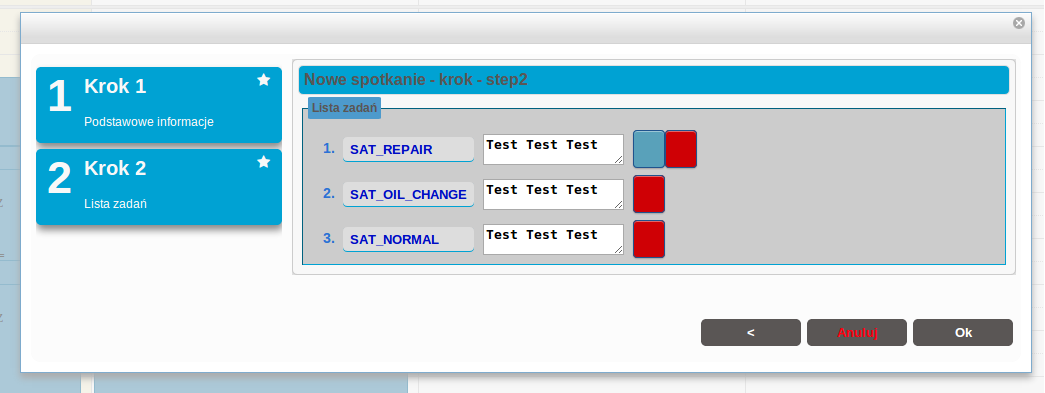
\includegraphics[width=1.0\textwidth]{images/newAppointment_step2}
		\caption[Kreator nowego spotkania - krok 2]{
			Kreator nowego spotkania - krok 2, źródło: opracowanie własne
		}
		\label{app:wizard_newAppointment_step2}
	\end{figure}
	\begin{figure}[H]
		\centering
		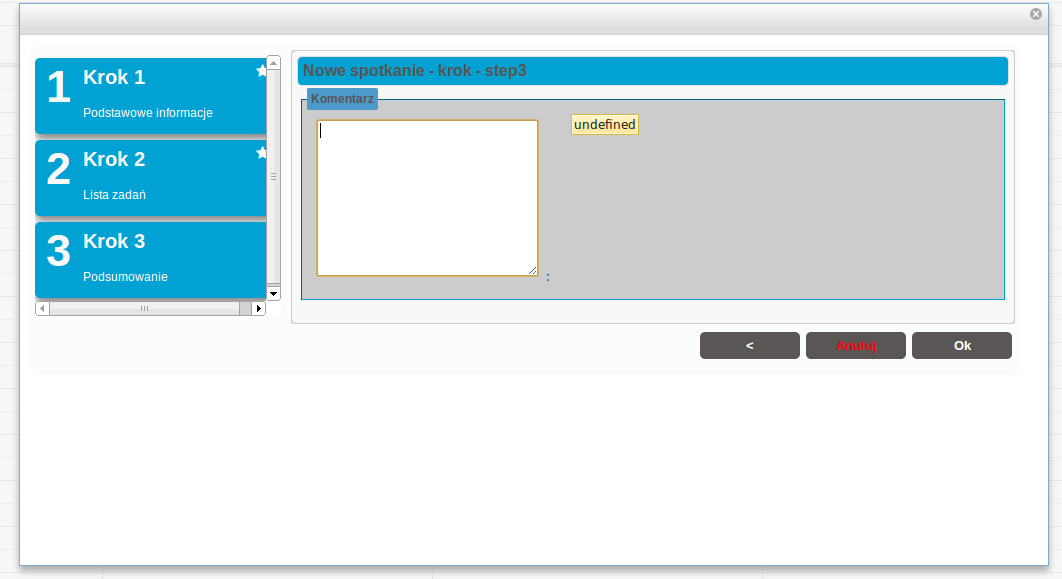
\includegraphics[width=1.0\textwidth]{images/newAppointment_step3}
		\caption[Kreator nowego spotkania - krok 3]{
			Kreator nowego spotkania - krok 3, źródło: opracowanie własne
		}
		\label{app:wizard_newAppointment_step3}
	\end{figure}		
	
	Dane wejściowe są walidowane pod kątem logiki biznesowej:
	\begin{itemize}
		\item termin spotkania:
		\begin{itemize}
			\item podane godziny (oraz czas) muszą mieścić się w wybranym zakresie [7-21],
			\item koniec spotkania nie może nastąpić później niż jego początek,
			\item zbyt krótkie (30 minut) oraz zbyt długie (10 dni),
			\item pokrywa się z co najmniej jednym spotkaniem dla mechanika wybranego jako wykonawca
		\end{itemize} 
		\item wybrany samochód:
		\begin{itemize}
			\item jeśli z właścicielem samochodu powiązane są jakiekolwiek problematyczne informacje, wyświetlane jest ostrzeżenie
		\end{itemize}
	\end{itemize}